% Created 2024-12-02 Mon 19:57
% Intended LaTeX compiler: xelatex
\documentclass[11pt]{article}
\usepackage{graphicx}
\usepackage{longtable}
\usepackage{wrapfig}
\usepackage{rotating}
\usepackage[normalem]{ulem}
\usepackage{capt-of}
\usepackage{hyperref}
\input{~/Preamble/preamble.tex}
\author{Wolfgang Rautenberg}
\date{\today}
\title{\zallman A Concise \\
\zallman Introduction\\
\zallman to\\
\zallman Mathematical \\
\zallman Logic\\
}
\hypersetup{
 pdfauthor={Wolfgang Rautenberg},
 pdftitle={\zallman A Concise \\
\zallman Introduction\\
\zallman to\\
\zallman Mathematical \\
\zallman Logic\\
},
 pdfkeywords={},
 pdfsubject={},
 pdfcreator={Notes Taken by Dendy Li}, 
 pdflang={English}}
\begin{document}

\maketitle
\tableofcontents

\newpage
\section{Propositional Logic}
\label{sec:orgfc78bf7}
Overview:

\textbf{Boolean functions and boolean formula}
\begin{center}
\begin{tikzpicture}
\tikzstyle{line} = [draw, -latex']
\node[align = center] (model)
{\begin{tabular}{rc}
\textbf{Propositional valuation} & \\
\textbf{Realization} & \(\omega : \text{PV} \to \{0,1\}\) \\
\textbf{Propositional Model} &
\end{tabular}
};

\node[align = center, right = of model] (boolean)
{\textbf{Boolean Function:} \( f : \{0,1\}^n \to \{0,1\} \)};

\node[align = center, below = of model] (extend)
{By recursive definition of \textbf{Formulas}, extend \(\omega\) to:\\
\( \bar{\omega} : \varphi \to \{0,1\} \), \( \varphi \in F_n\).};

\node[below = of boolean] (space1)
{};

\node[align = center, below = 2cm of $(space1)!0.5!(extend)$] (recursive)
{\textbf{Fact: } \\
Assign a truth value to a formula \( \Leftrightarrow \) Assign a true value at all occurance of the PV};

\path [draw] (model) -- (extend);
\path [draw] (extend) -- (recursive);
\path [draw] (recursive) edge["\(\bar{\omega}\varphi = f(\omega \vec{p})\)"'] (boolean);

\end{tikzpicture}
\end{center}

\textbf{Semantic of Propositional Logic}
\begin{center}
\begin{tikzpicture}
\tikzstyle{line} = [draw, -latex']

\node[align = center] (equiv)
{\textbf{Semantic Equivalence:} \\
\(\alpha \equiv \beta \Leftrightarrow \omega\alpha \equiv \omega\beta\)};

\node[align = center, below = 2cm of equiv] (replace)
{\textbf{Replacement Theorem:} \\
\(\alpha \equiv \alpha' \Rightarrow \varphi \equiv \varphi'\), \\
\( \varphi' \) is obtained from \( \varphi \) by replacing occurence of  \( \alpha \) in \( \varphi \), by \( \alpha' \).};

\node[align = center, right = of $(equiv)!0.5!(replace)$] (Rep)
{\textbf{Motivation:} \\
If every boolean functions can \\
be represented by a boolean formula?};

\node[align = center, below = 2cm of $(Rep)!0.5!(replace)$] (DNF)
{Every boolean function \( f \) can be represented by DNF \( \alpha_f \), i.e. \\
\( \alpha_f := \lor_{f\vec{x} = 1} p_1^{x_1} \land \cdots \land p_n^{x_n}\), \\
where \( (x_1, \dots, x_n) \in \{0,1\}^n \), \( p_i^0 := p_i, p_i^1 := \neg p_i \).};

\node[align = center, below = of DNF] (funcomp)
{\textbf{Functional Complete:} \\
Logical signature is functional complete it can represent every boolean functions.};

\path [draw] (equiv) -- (replace);
\path [draw] (replace) -- (DNF);
\path [draw] (DNF) -- (funcomp);

\end{tikzpicture}
\end{center}

\newpage
\textbf{Logical Consequence and its properties}

\begin{center}
\begin{tikzpicture}
\tikzstyle{line} = [draw, -latex']

\node[align = center] (model)
{\textbf{Model:} \\
If \( \omega\alpha = 1 \), \( \omega \) is a model of \( \alpha \), \\
or \( \omega \) satisfies \( \alpha \), denote as \( \omega \models \alpha \). \\
This definition can naturally be extended to \\
a set of formulas \( X \). \\
\( \models \) is the satisfiability relation. \\
\( \alpha (X) \) is satisfiable if there exists a model.};

\node[align = center, below = of model] (logc)
{\textbf{Logical Consequence:} \\
If \( \omega \models X \), then \( \omega \models \alpha \). \\
We say \( \alpha \) is a logical consequence of \( X \).};

\node[align = center, right = of model] (tautocontra)
{\textbf{Tautology:} \\
If all \( \omega \) satisfy \( \alpha \), \\
\( \alpha \) is a tautology. \\
\textbf{Contradiction:} \\
If all \( \omega \) don't satisfy \( \alpha \), \\
\( \alpha \) is a contradiction. \\
\textbf{Negation of a tautology isn't a contradiction.}};

\node[align = center, below = of logc] (proplogc)
{\textbf{Basic properties of \( \models \):} \\
\begin{tabular}{l}
(R) : \textbf{Reflexive} \\
(M) : \textbf{Monotone} \\
(T) : \textbf{Transitive} \\
\end{tabular}};

\node[align = center, right = of proplogc] (factontau)
{\textbf{Fact of Tautology:} \\
Tautologies of the form \( \alpha \lor \neg\alpha \) is implied by \( p \lor \neg p \).};

\node[align = center, below = of factontau] (substitution)
{(S) : \textbf{Invariance Substitution}};

\node[align = center, below = of proplogc] (compact)
{(F) : \textbf{Finitary:} \\
\( X \models \alpha \Rightarrow X_0 \models \alpha \), \\
\( X_0 \subseteq X \), \( X_0 \) finite.};

\node[align = center, below = 2cm of $(compact)!0.5!(substitution)$] (general)
{\( \models \) shares the properties (RMTS) with almost all classical / non classical Logical systems. \\
A propositional consequence relation \( \vdash \), is a relation \\
between sets of formulas and formulas of a given FOL \( \calf \), \\
with properties corresponds to (RMTS).};

\node[align = center, below = of general] (deduction)
{\textbf{Deduction Theorem:} \\
\( X, \alpha \models \beta \Rightarrow X \models \alpha \to \beta\).};

\path [draw] (model) -- (logc);
\path [draw] (logc) -- (proplogc);
\path [draw] (deduction) -- (general);
\path [draw] (proplogc) -- (factontau);
\path [draw] (factontau) -- (substitution);
\path [draw] (substitution) -- (general);
\path [draw] (factontau) -- (tautocontra);
\path [draw] (model) -- (tautocontra);

\end{tikzpicture}
\end{center}

\textbf{Syntax of Complete Calculus for \(\models\):}

\begin{center}
\begin{tikzpicture}
\tikzstyle{line} = [draw, -latex']

\node[align = center] (prove)
{\textbf{Derivability Relation \( \vdash \):} \\
\( \vdash \) is a relation between set of formulas and formulas. \\ If \( \vdash \) can applies to pair \( (X, \alpha) \), denote as \( X \vdash \alpha \), \\ call \( \alpha \) is a derivation from \( X \). Otherwise \( X \not\vdash \alpha \). \\ \( (X, \alpha) \) is called \textbf{sequent} w.r.t. Gentzen. \\
\textbf{Calculus on \( \vdash \):} \\
\begin{tabular}{l}
(1) : A functional complete logical signature \(\{\land, \neg\}\); \\
(2) : 6 basic rules which are designed for completeness, \\ these 6 rules will be showed in the equivalent definition below; \\
(3) : Provable rules / Derivable rules are the rules \\ can be intefere from (1) (2).\end{tabular} \\
\textbf{Remark:} \( \frac{X, \neg\alpha \vdash \beta, \neg\beta}{X \vdash \neg\alpha}\).};

\node[align = center, below = of prove] (formalprove)
{\textbf{Derivability Relation \( \vdash \) (Equivalent Definition):} \\
Smallest relation \( \subseteq \mathfrak{B}\calf \times \calf \) and \\ closed under the following 6 rules: \\
\begin{tabular}{ll}
\( \frac{ }{\alpha \vdash \alpha} \) & \( \frac{X \vdash \alpha}{X' \vdash \alpha}, X \subseteq X' \). \\
\( \frac{X \vdash \alpha, \beta}{X \vdash \alpha \land \beta} \) & \( \frac{X \vdash \alpha \land \beta}{X \vdash \alpha, \beta} \) \\
\( \frac{X \vdash \neg \alpha, \alpha}{X \vdash \beta} \) & \( \frac{\alpha, X \vdash \beta | X, \neg \alpha \vdash \beta}{X \vdash \beta} \)
\end{tabular}};

\node[align = center, right = of prove] (models)
{\textbf{Consequence Relation \( \models \)}};

\node[align = center, below = of formalprove] (conventionofprove)
{\textbf{Conventions of \( \vdash \):} \\
\begin{tabular}{l}
\( X, \alpha \vdash \alpha \Leftrightarrow X \cup \alpha \vdash \alpha \); \\
\( X \vdash \alpha, \beta \Leftrightarrow X \vdash \alpha \text{and} X \vdash \beta \); \\
The syntax is of the form \( \frac{\text{Premises}}{\text{Inference}}\).
\end{tabular}};

\node[align = center, below = of models] (syntacticmeaning)
{\textbf{Syntactical Meaning of \( X \vdash \alpha \):} \\
\( (X, \alpha) \) can be obtain \\ from stepwise application.};

\node[align = center, below = of syntacticmeaning] (derivation)
{\textbf{Derivation:} \\
Derivation is the records of the \\ stepwise application process. \\
\textbf{Derivation(Formal):} \\
A derivation of \( (X, \alpha) \) \\ is a tuple \( (S_0, \dots, S_{n-1}, S_n) \) \\ where \( S_n = (X, \alpha) \), each of \( S_i \) \\ is obtained by the following rules: \\
\begin{tabular}{l}
(1) IS ; \\
(2) Basic rules applies on \( S_k, k \leq i \).
\end{tabular}};

\path [draw] (syntacticmeaning) -- (models);
\path [draw] (derivation) -- (syntacticmeaning);
\path [draw] (prove) -- (formalprove);
\path [draw] (formalprove) -- (conventionofprove);
\path [draw] (prove) edge["\tiny{identical with}"] (models);

\end{tikzpicture}
\end{center}

\textbf{Semantics of \(\vdash\):}

\begin{center}
\begin{tikzpicture}
\tikzstyle{line} = [draw, -latex']

\node[align = center] (induction-on-property) at (0,0)
{\textbf{Property of sequents:} \\
\( \cale \) is a property of sequents, \\ i.e. \( \cale \) can apply on the pair \( (X, \alpha) \). \\
\textbf{Induction on property:} \\
Let \( \cale \) be a property closed under \( \vdash \), \\ then \( X \vdash \alpha \) implies \( \cale(X,\alpha) \). \\ \( \cale := \models \) is a good example.};

\node[align = center, right = of induction-on-property] (semantic-soundness)
{\textbf{Soundness(Semantic):} \\
\( \vdash \subseteq \models \)};

\node[align = center, below = 2cm of $(induction-on-property)!0.5!(semantic-soundness)$] (connect)
{With induction on property, we will deduce \\ a symmetric process \\ which builds a relation of \( \vdash \) and \( \models \).};

\node[align = center, below = of connect] (finiteness-theorem-prove)
{\textbf{Finiteness theorem for \( \vdash \):} \\
If \( X \vdash \alpha \), then exists finite \( X_0 \subseteq X \) with \( X_0 \vdash \alpha \).};

\node[align = center, below left = of finiteness-theorem-prove, text width = 0.3 \textwidth] (consistent)
{\textbf{Consistent:} \\
\( X \subseteq \calf \) is consistent if \( X \vdash \alpha \) for all \( \alpha \); else consistent. \\
\( X \subseteq \calf \) is maximal consistent if \( X \) is consistent and any \( X \subseteq Y \), is inconsistent.};

\node[align = center, below = of consistent] (top-down-bottom-up)
{\( C^+ : X \vdash \alpha \Leftrightarrow X, \neg\alpha \vdash \bot \); \\
\( C^- : X \vdash \neg\alpha \Leftrightarrow X, \alpha \vdash \bot \).};

\node[align = center, right = of consistent] (Lindenbaum)
{\textbf{Lindenbaum's theorem:} \\
Every consistent set \( X \) can be extended \\ to a maximally consistent set \( X' \supseteq X \)};

\node[align = center, below right = of consistent] (property-max-consistent)
{\textbf{Properties of maximal consistent:} \\
\begin{tabular}{l}
(1) : \( X \vdash \neg\alpha \Leftrightarrow X \not\vdash \alpha \); \\
(2) : Maximally consistent set \( X \) is satisfiable.
\end{tabular}};

\node[align = center, below = of property-max-consistent] (completeness)
{\textbf{Completeness theorem:} \\
\( X \vdash \alpha \Leftrightarrow X \models \alpha \).};

\node[align = center, below = of completeness] (result-completeness)
{\textbf{Results of completeness theorem:} \\
\begin{tabular}{l}
(1) : If \( X \vdash \alpha \), then fintite \( X_0 \subseteq X \), \( X_0 \models \alpha \). \\
(2) : A set \( X \) is satisfiable then each finite subset of \( X \) is satisfiable.\end{tabular}};

\path [draw] (property-max-consistent) -- (completeness);
\path [draw] (completeness) -- (result-completeness);
\path [draw] (property-max-consistent) -- (consistent);
\path [draw] (induction-on-property) edge["induce"] (semantic-soundness);
\path [draw] (finiteness-theorem-prove) -- (connect);
\path [draw] (consistent) -- (finiteness-theorem-prove);
\path [draw] (consistent) -- (top-down-bottom-up);

\end{tikzpicture}
\end{center}

\textbf{Hilbert Calculi:}

\begin{center}
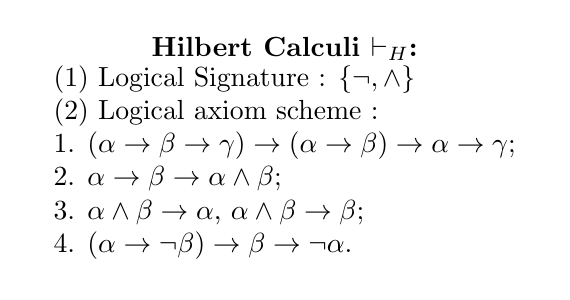
\begin{tikzpicture}
\tikzstyle{line} = [draw, -latex']

\node[align = center] (Hilbert)
{\textbf{Hilbert Calculi \( \vdash_H \):} \\
\begin{tabular}{l}
(1) Logical Signature : \( \{\neg, \land\} \) \\
(2) Logical axiom scheme : \\
1. \( (\alpha \to \beta \to \gamma) \to (\alpha \to \beta) \to \alpha \to \gamma \); \\
2. \( \alpha \to \beta \to \alpha \land \beta \); \\
3. \( \alpha \land \beta \to \alpha \), \( \alpha \land \beta \to \beta \); \\
4. \( (\alpha \to \neg \beta) \to \beta \to \neg \alpha \).
\end{tabular}};

\end{tikzpicture}
\end{center}
\subsection{Boolean Functions and Formulas}
\label{sec:org5897f19}
\subsubsection{What is Prositional Language?}
\label{sec:orgd5acf80}
\begin{definition}[n-ary Boolean Functions]
\(f:\{0,1\}^n\to\{0,1\}\) is called an \(n\)-ary Boolean function or Truth function.
\end{definition}

\begin{proposition}
\(n\)-ary Boolean function \(f\) has \(2^n\) tuples in its \textbf{domain}, this gives \(2^{2^n}\) ways to construct an \(n\)-ary Boolean function.
\end{proposition}

\begin{definition}
We denote the totality above as \(\mathbf{B}_n\), that is \(\mathbf{B}_n=2^{2^n}\).
\end{definition}

\begin{definition}[Propositional Language(defined by induction)]
Given a set of logic symbols(\emph{Logical signature}) and a set of variables. We define propositional language \(\mathfrak{F}\) inductively:
\begin{enumerate}
\item one-element strings are formulas(\emph{Prime Formulas}).
\item If \(\alpha, \beta\) are all formulas then \(\alpha \circ \beta\) here \(\circ\) refers to binary Boolean Functions and \(\lnot\alpha\in S.\)
\end{enumerate}
\end{definition}


Based on set theory we also have another definition:
\begin{definition}[Propositional Language(defined in set-theoretical way)]
Propositional Language \(\mathfrak{F}\) is the smallest set of all \textbf{String} \(S\) built from \emph{logic symbols} and \emph{propsitional variables}, satisfying the following properties:
\begin{itemize}
\item[f1] \(p_1,\dots\in S.\)
\item[f2] \(\alpha,\beta\in S\) they are closed under the binary Boolean function and unary Boolean function.
\end{itemize}
\end{definition}

\begin{definition}[Formula]
A string in a propositional language is a formula.
\end{definition}

\begin{examplle}[ ]
For Boolean Signature we have the Boolean formulas.
\end{examplle}

Worth noticing that we don't use parentheses for the unary operation.

\textbf{Now we let \(\mathfrak{F}\) to be the set of all Boolean formulas.}

For convention we obey the following rules:
\begin{enumerate}
\item Omit the outside parentheses.
\item If order of the logic connectives makes the formula no ambiguity without parentheses then we omit the parentheses.
\item Multiple use of \(\rightarrow\) we associate to the right; multiple use of other binary connectives we associate them to the left.
\end{enumerate}

\textbf{In arithmetic one used to associate to the left but \(x^{y^z}\) is an example of associate to the right.}

\begin{theorem}[Induction principle for formulas]
Let \(\Epsilon\) be a property of strings(We write \(\Epsilon\psi\) to represent \(\Epsilon\) is a property of string \(\psi\)), such that(If one can show):
\begin{itemize}
\item \(\Epsilon\pi\) for prime formual \(\pi\),
\item \(\Epsilon\alpha, \Epsilon\beta\), then the formulas building from \(\alpha, \beta\) also have this property.
\end{itemize}
Then \(\Epsilon\) holds for all formula.
\end{theorem}

\textbf{Some Language notation:}
\begin{itemize}
\item \textbf{Such that means suppose to show, means the goal is\ldots{}}

\item \textbf{Compound is the words from chemestry, which means that many different kinds of elements together form sth, this sth is so-called compound.}
\end{itemize}

\begin{theorem}[Unique reconstruction property]
If \(\alpha, \beta\) where \(\alpha \circ \beta\) construct \(\varphi\), then \(\alpha, \beta\) are uniquely determined.
\end{theorem}

This property looks very weird since it somehow have the idea of the free generation and have some idea of unique readability theorem.

\begin{definition}[Inductive defintion of subformula]
\begin{itemize}
\item subformula of prime formula is itself
\item subformula of \(\neg \alpha\) is \(\{\neg \alpha\} \cup\) subformula of \(\alpha\)
\item for boolean signature just the natural way: itself and subformulas of the component.
\end{itemize}
\end{definition}

\textbf{By arithmetic one emphersize the numbers and the operations on it.}

\begin{definition}[Propositional valuation(Realization of propositional model)]
A propositional valuation \(\omega\) is a function \(\omega:PV \to \{0,1\}\).
\end{definition}

\textbf{Stipulation: a rule must be follow or sth must be done.}

we can extend the valuation in natural inductive way:
\begin{itemize}
\item \(\omega\alpha \circ \beta = \omega\alpha \circ \omega\beta\)
\item \(\omega\neg\alpha = \neg\omega\alpha\)
\end{itemize}

By the extension we can talk about the valuation of formula \(\varphi\).

For the next part we will talk about the connection between boolean functions and boolean formulas
\subsubsection{Correspondence between boolean formulas and boolean functions}
\label{sec:org8c01bcf}
\subsection{Semantic Equivalence and Normal Forms}
\label{sec:orgca3f5ef}
\section{Predicate Logic}
\label{sec:orgae57b74}
\subsection{Overview of the basical objects}
\label{sec:orgfc0c572}

\begin{center}
\begin{tikzpicture}
\tikzstyle{line} = [draw, -latex']

\node[align = center] (symbols)
{\begin{tabular}{l}
\textbf{Extralogical Structure \( L \):} \\
Constant symbols, function symbols, relation symbols. \\
e.g. in group theory \(\{ \circ, e\}\). \\

\textbf{\( L \)- Structure \(\cala\):} \\
\( (A, L^{\cala}) \), \( A \) is the domain of \( \cala \), \\
\( L^{\cala} \) consists of the interpretation of the extralogical structure. \\
\end{tabular}};

\node[align = center, below = of symbols] (alphabet)
{\begin{tabular}{l}
\textbf{Alphabet of \( L \):} \\
The alphabet of \( L \) consists of \( L \), \\
logical symbols and varibales.

\textbf{Strings of \( L \):} \\
\( \cals := \{ \text{The set of all strings from } L \} \).
\end{tabular}
};

\node[below = of alphabet] (spaceA)
{};

\node[align = center, right = of spaceA] (recursive)
{\begin{tabular}{l}
\textbf{Recursive definition of:} \\
Terms \\
Prime Formulas \\
Varibales
\end{tabular}};

\node[align = center, below = of spaceA] (FOL)
{\begin{tabular}{l}
\textbf{\( \call \) := \{The set of all formulas determined by \( L \).\}}\\
\textbf{\( \call^0 \) := \{The set of all the sentences\}.} \\
\textbf{Sentences: } Formula with no free variable.
\end{tabular}};

\node[align = center, below = of FOL] (Lstructure)
{\( L \)- structure for extralogical symbol \( L \), \\
naturally become \( \call \)- structure, \\
with the recursive definition of terms and formulas.};

\path [line] (symbols) -- (alphabet);
\path [line] (alphabet) -- (FOL);
\path [line] (FOL) -- (Lstructure);



\end{tikzpicture}
\end{center}
\subsection{Mathematical Structures}
\label{sec:org6d3982a}

\begin{definition}["Specific" Structure and related definition]
For structure \(\mathfrak{A}\) we have the following description:

\begin{center}
\begin{tabular}{ccc}
Notations & \(A\): Domain & relations \(r\), operations \(f\), constant \(c\)\\

Descriptions & finite(infinite) structure & relation(algebraic) structure
\end{tabular}
\end{center}

\begin{itemize}
\item Relation structure has no operation and constant
\item Algebraic structure has no relation
\end{itemize}
\end{definition}

\textbf{We want to study the class of structures, so we need a ``connection'' which enables us to talk about a class of structures.}

\begin{definition}[Extralogical Signature]
A finite set \(L\) consisting of relation, operation, and constant symbols of given arity, is a (extralogical) structure.
\end{definition}

\begin{definition}[Closed under operations]
\(\forall a \in A^n \Rightarrow fa \in A\).
\end{definition}

\begin{definition}[Restriction to a subset of domain]
\textbf{Restriction for Relation:}
\begin{itemize}
\item Intersect product sets
\end{itemize}
\textbf{Restriction for Operations:}
\begin{itemize}
\item Closed under operations w.r.t. the subset which we want to restrict on.
\end{itemize}
\end{definition}

\begin{definition}[Substructure]
Let \(\mathfrak{B}\) be an L-Structure, \(A \subset B\) nonempty and closed
under all operations of \(B\) and inherits all the interpratations of constant of \(B\).
\end{definition}

\begin{proposition}[Common properties of binary operations and binary relations]
\textbf{Properties for binary operations:}
\begin{itemize}
\item Commutivity;
\item Associativity;
\item Idempotent: \(a \circ a = a\);
\item Invertible: \(\forall a,b, \exists x,y \Rightarrow a \circ x = b \land y \circ a = b\).
\end{itemize}

\textbf{Properties for binary relations:}
\begin{itemize}
\item reflexive and irreflexive;
\item symmetric and antisymmetric;
\item transitive;
\item connex(Trinity).
\end{itemize}
\end{proposition}
\subsection{Syntax of Elementary Languages}
\label{sec:org12bf8a7}

\begin{center}
\begin{tikzpicture}
\tikzstyle{line} = [draw, -latex']

\node [align = center] (Term)
{\textbf{Term} \\
\begin{tabular}{l}
1. \textbf{Prime Term} : Variables and constants \\
2. \textbf{Compound of functional symbol and terms}
\end{tabular}};

\node[right = of Term, align = center] (Formula)
{\textbf{Formula} \\
\begin{tabular}{l}
1. \textbf{Terms} \\
2. \textbf{Compound of relation and terms} \\
3. \textbf{Compound of logical connectives} \\ \textbf{and formulas}
\end{tabular}};

\node[below = of Formula] (Variables)
{\begin{tabular}{l}
1. \textbf{Variable} \\
2. \textbf{Free Variable} \Rightarrow \textbf{Sentences}\\
3. \textbf{Bounded Variable}
\end{tabular}
};


\path [line] (Term) -- (Formula);
\path [line] (Formula) -- (Variables);

\end{tikzpicture}
\end{center}

\textbf{Goal: We want to delimit(determine the limit) the theoretical framework which enables us to precisely talk about mathematical structures}

This goal arise the definition of object language.
\begin{definition}[Object Language]
Object Language is the language can be described by metalanguage.
\end{definition}

\begin{definition}[Object(w.r.t. object language)]
Objects are formalized elements of the language.
\end{definition}

To formalize interesting properties of a structure, one need the following things:

\begin{definition}[Individual Variables(Informal)]
Individual variables are a ``place-holder'' with a predicate letter. It stands for unspecified argument of the predicate.
\end{definition}

\begin{definition}[Extralogic Structures(w.r.t. the given language)]
Sufficient number of relations, funcitons and constant.
\end{definition}

The language with the two features above is the first order language or elementary languages, now we give a formal definiton.

\begin{definition}[First-order language(Informal)]
First-order language is a set consists of the following type of subsets:
\begin{itemize}
\item Alphabet
\begin{itemize}
\item Individual variables(Var): countably many variables.
\item Extralogic structures
\end{itemize}
\item Syntax of first-order logic
\item Semantics of first-order logic
\end{itemize}
\end{definition}

\textbf{Remark:}
\begin{itemize}
\item \textbf{One can only differ two first-order language by the Extralogical Structures.}
\item \textbf{Individual Variables here often denotes by \(x,y,z,\dots\).}
\end{itemize}

\begin{definition}[Alphabet]
Alphabet is the set of basic symbols of a first-order language determined by a (extralogical) signature \(L\).
\end{definition}
\section{Gödel's Completeness Theorem}
\label{sec:org78074cd}

\begin{center}
\begin{tikzpicture}
\tikzstyle{line} = [draw, -latex']

\node[align = center] (Deduction)
{
\begin{tabular}{l}
\textbf{Natural Deduction:} Gentzen's type \(\vdash_G\)\\
\textbf{Hilbert Calculi:} Modus ponens \(\vdash_H\)
\end{tabular}};

\node[align = center, right = of Deduction] (CompletenessTheorem)
{\textbf{Gödel's Completeness Theorem} \\
\begin{tabular}{l}
1. \(\vdash_H = \models\) \\
2. \(\vdash_G = \models\) \\
3. \textbf{Finiteness Theorem:} \\ \(X \models \alpha \Rightarrow  X_0 \models \alpha, X_0 \subseteq X, X_0 \text{ finite.}\) \\
4. \textbf{Compactness Theorem(Syntactic):} \\ Any set of first order formula \(X\) is satisfiable \(\Rightarrow\) \\ Every finite subset of \(X\) is satisfiable.
\end{tabular}
};

\node[align = center, below = of CompletenessTheorem] (Complete)
{A theory is \textbf{complete} if it is consistent \\ and has no proper consistent extension.};

\path [draw] (Deduction) -- (CompletenessTheorem);
\path [draw] (CompletenessTheorem) -- (Complete);

\end{tikzpicture}
\end{center}
\section{Incompleteness and Undecidability}
\label{sec:org141a500}
Overview:
\begin{center}\begin{tikzcd}
\text{Recursive and Primitive Recursive Functions} \ar[d] & \text{Arithmatic on syntax and formal proofs} \ar[dl]\\
\text{Representability of recursive functions} \ar[d] & \\
\text{First Incompleteness Theorem} \ar[d] \ar[dr] \\
\text{Decidability and Undecidability} & \text{First-order arithmetical hierachy}
\end{tikzcd}\end{center}

Gödel's first incompleteness theorem informal description:
\textbf{Basic Assumption:}
\begin{center}\begin{tikzcd}
\mathcal{T}:\text{Axiomatic theory} \ar[r,"\text{describe}"] & \mathcal{A}:\text{Given domain of objects} \\
\mathcal{L}:\text{Language of} \mathcal{T} \ar[u,"\text{Internal encoding of syntax of}\mathcal{L}"]
\end{tikzcd}\end{center}

\textbf{Result:}
Sentence \(\gamma:\)``I(\(\gamma\)) am provable in \(\mathcal{T}\)'' is true in \(\mathcal{A}\) but unprovable in \(\mathcal{T}\)

This result is kind of like the liar paradox. ``I will not died because of fire.'' This is true because within the rule I will not die. This is unprovable because we can't make sure the semantic of this sentence within the rules.
\subsection{Recursive and Primitive Recursive Functions}
\label{sec:orgbd23541}

\begin{definition}[Partial Function]
Let \(X,Y\) be sets, \(S\subset X\). \(f:S\to Y\) is a partial function from \(X\to Y\).
\end{definition}

\textbf{Difference between primitive recursive functions and recursive functions}
\begin{itemize}
\item Primitive recursive functions are from primitive recursive functions with one input.
\item Recursive function: Partial functions take finite tuples of natural numbers and return a single natural number.
\end{itemize}

\begin{proposition}[ ]
Primitive recursive function \(\subset\) Recursive function \(\subset\) Partial recusive function.
\end{proposition}

\begin{definition}[Halting Problem]

\end{definition}

\textbf{Goal: Code Undecidability into logic}

\begin{definition}[Computation]
Computation is a sequence of configuration of addition mechine.
\end{definition}

\textbf{Remark: Here configuration means the current states.}
\section{Kappa-categorical}
\label{sec:org36b97e1}
\begin{definition}[Kappa-categorical]
We say a theory is \(\aleph_0\)-categorical if any countable infinite models are isomorphic.
\end{definition}
\end{document}
